%!Tex Root = ../main.tex
% ./Packete.tex
% ./Design.tex
% ./Deklarationen.tex
% ./Vorbereitung.tex
% ./Aufgabe1.tex
% ./Aufgabe3.tex
% ./Aufgabe4.tex
% ./Bonus.tex

\section{Aufgabe 2}

\setcounter{task}{1}

\begin{frame}[allowframebreaks]{Exercise 2}{Isomorphisms}
  \begin{requirementsnoinc}
    % \begin{definition}{Isomorphism}
    % \end{definition}
    \begin{itemize}
      \item \alert{Isomorphism:} Two Graphs $G$ and $H$ are \alert{isomorphic} if there exists a \alert{bijection} $\varphi: V(G) \to V(H)$ such that  $uv\in E(G) \Leftrightarrow \varphi(u)\varphi(v) \in E(H)$. In which case, we write $G\cong H$.
      \begin{itemize}
        \item because of the \alert{bijection} both graphs $G$ and $H$ must have the \alert{same number} of \alert{vertices}
        \item because both graphs $G$ and $H$ need to have the \alert{\enquote{same neighbours}} (have to satisfy two corresponding relations) they must have the \alert{same number} of \alert{edges}. To be clear, it does also hold: $uv\not\in E(G) \Leftrightarrow \varphi(u)\varphi(v)\not\in E(H)$
        \item two \alert{unlabbeled graphs} are isomorphic if they would be isomorphic under \alert{any} \alert{labelling} of their vertices
      \end{itemize} 
      \ctikzfig{example_isomorphism}
    \end{itemize}
  \end{requirementsnoinc}
  \begin{requirementsnoinc}
    \begin{itemize}
      \item \alert{bijective:} injective + surjective, every element from $B$ has \alert{exactly} one partner in $A$ ($\forall b \in B \exists ! a \in A:(a, b) \in R$)
      \begin{itemize}
        \item $R\subseteq A\times B$
        \item \alert{injektiv / left-unique:} Every element from $B$ has \alert{at most} one partner in $A$ ($\forall b \in B \forall a, c \in A:(a, b) \in R \wedge(c, b) \in R \Rightarrow a=c$, \textit{mnemonic:} \enquote{a injection shouldn't be made twice at the same spot})
        \item \alert{surjektiv / right-total} Every element from $B$ has \alert{at least} one partner in $A$ ($\forall b \in B \exists a \in A:(a, b) \in R$)
        \item \alert{left-unique} and \alert{right-total} both describe relationships focusing on the \alert{codomain} $B$ while their correspondings counterparts for functions \textit{right-unique } (partial function, $\forall a \in A \forall b, d \in B:(a, b) \in R \wedge(a, d) \in R \Rightarrow b=d$) and \textit{left-total } (german: \enquote{Multifunktion}, $\forall a \in A \exists b \in B:(a, b) \in R$) focus on the domain $A$ (\textit{function:} Every element from $A$ has \enquote{exactly} one partner in $B$ ($\forall a \in A \exists ! b \in B:(a, b) \in R$)
      \end{itemize}
    \end{itemize}
  \end{requirementsnoinc}
  \begin{solutionnoinc}
    \begin{columns}
      \begin{column}{0.5\textwidth}
        \ctikzfig{2a_1}
      \end{column}
      \begin{column}{0.5\textwidth}
        \ctikzfig{2a_2}
      \end{column}
    \end{columns}
    \vspace{0.5cm}
    \begin{enumerate}
      \item look at the \alert{number} of \alert{vertices} and \alert{edges} $\rightarrow$ both $8$ vertices and $16$ edges
      \item[]
      \item[]
    \end{enumerate}
  \end{solutionnoinc}
  \begin{solutionnoinc}
    \begin{columns}
      \begin{column}{0.5\textwidth}
        \ctikzfig{2a_1_sol_2}
        % ./figures/2a_1_sol_2.tikz
      \end{column}
      \begin{column}{0.5\textwidth}
        \ctikzfig{2a_2_sol_2}
        % ./figures/2a_2_sol_2.tikz
      \end{column}
    \end{columns}
    \vspace{0.5cm}
    \begin{enumerate}
      \item look at the \alert{number} of \alert{vertices} and \alert{edges} $\rightarrow$ both $8$ vertices and $16$ edges
      \item look at \alert{degree} of vertices
      \item[]
    \end{enumerate}
  \end{solutionnoinc}
  \begin{solution}
    \begin{columns}
      \begin{column}{0.5\textwidth}
        \ctikzfig{2a_1_sol}
        % ./figures/2a_1_sol.tikz
      \end{column}
      \begin{column}{0.5\textwidth}
        \ctikzfig{2a_2_sol}
        % ./figures/2a_2_sol.tikz
      \end{column}
    \end{columns}
    \vspace{0.5cm}
    \begin{enumerate}
      \item look at the \alert{number} of \alert{vertices} and \alert{edges} $\rightarrow$ both $8$ vertices and $16$ edges
      \item look at \alert{degree} of vertices
      \item search for \alert{subgraphs} / \alert{cycles}
    \end{enumerate}
  \end{solution}
  \begin{requirementsnoinc}
    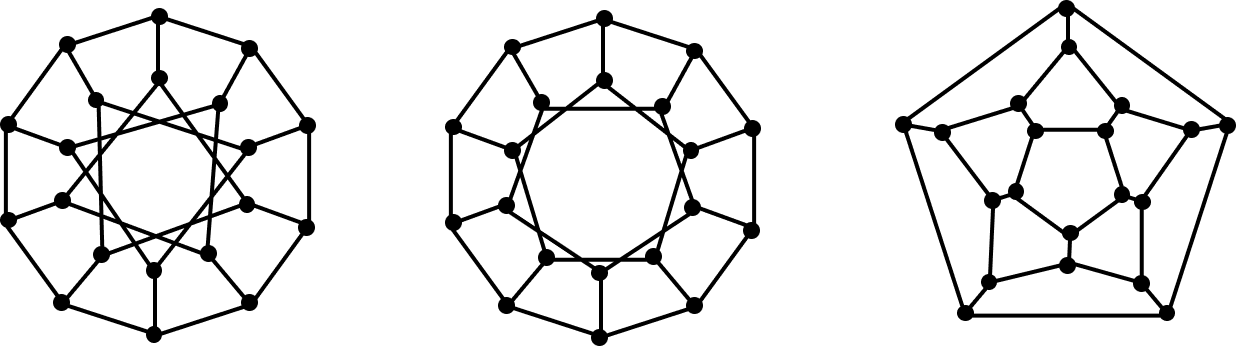
\includegraphics[width=\textwidth]{./figures/isomorphism2.png}
  \end{requirementsnoinc}
  \begin{solutionnoinc}
    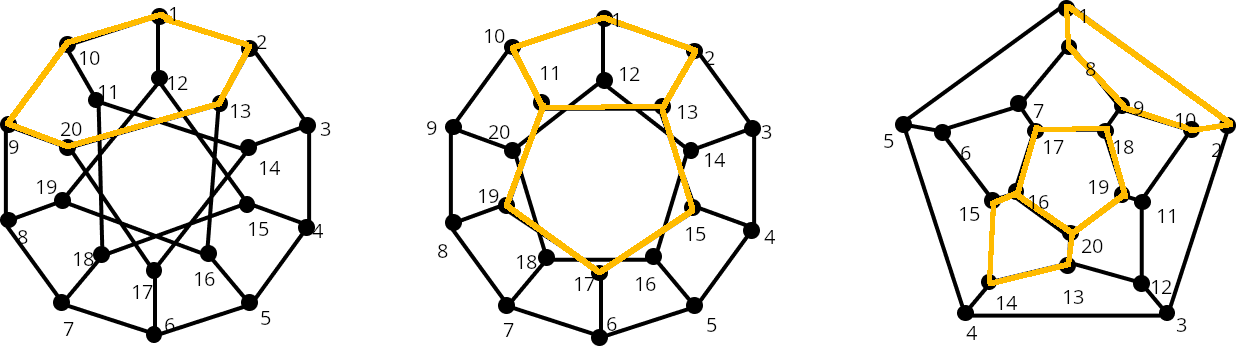
\includegraphics[width=\textwidth]{./figures/isomorphism2_sol.png}
    \setcounter{MaxMatrixCols}{20}
    \begin{itemize}
      \item $2$ and $3$ are \alert{isomorphic}
    \end{itemize}
  \end{solutionnoinc}
  \begin{solution}
    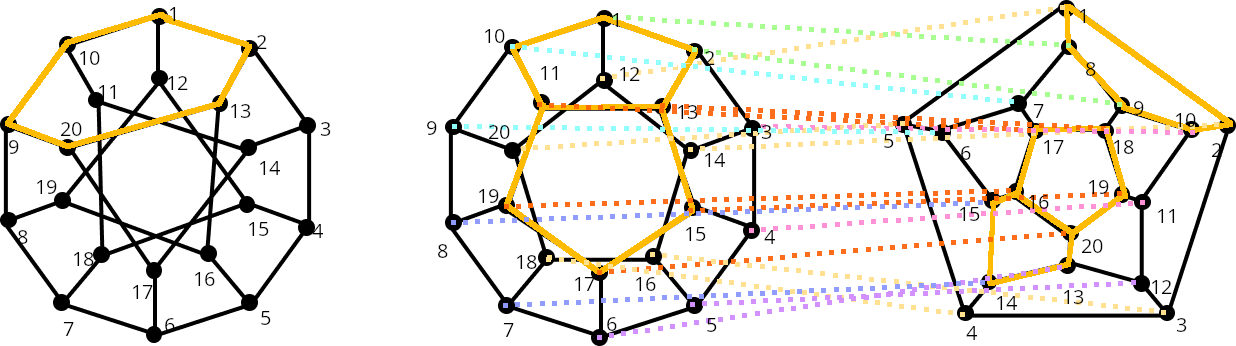
\includegraphics[width=\textwidth]{./figures/isomorphism2_sol_2.png}
    \setcounter{MaxMatrixCols}{20}
    \begin{itemize}
      \item \alert{Permutation}: 
    \end{itemize}
    \vspace{0.25cm}
    \[\pi := \begin{aligned}[t]
      \scriptsize
      \begin{pmatrix}
        1 & 2 & 3  & 4  & 5  & 6  & 7  & 8  & 9 & 10 & 11 & 12 & 13 & 14 & 15 & 16 & 17 & 18 & 19 & 20 \\
        8 & 9 & 10 & 11 & 12 & 13 & 14 & 15 & 6 &  7 & 17 &  1 & 18 &  2 & 19 &  3 & 20 &  4 & 16 &  5 \\
      \end{pmatrix}
    \end{aligned}\]
  \end{solution}
  \begin{example}
    \ctikzfig{example_isomorphism_2}
    \begin{itemize}
      \item \alert{fast method:} find \textit{corresponding vertices of same degree} and make sure the \enquote{neigbors} match up
      \item \alert{confirm isomorphism} between graphs by \alert{creating the isomorphism}
    \end{itemize}
  \end{example}
\end{frame}
